\documentclass[conference]{IEEEtran}

\usepackage{amsmath,amssymb}
\usepackage{booktabs}
\usepackage{graphicx}
\usepackage{hyperref}
\usepackage{array}
\usepackage{multirow}
\usepackage{xcolor}
\usepackage{tikz}
\usepackage{pgfplots}
\pgfplotsset{compat=1.18}
\usetikzlibrary{arrows.meta,shapes.geometric,positioning,fit,calc}

\graphicspath{{figures/new/main/}{figures/new/}{figures/legacy/}{figures/report/}}

\begin{document}

\title{TA-BRPL: Trust-Aware Backpressure RPL for Mitigating Sinkhole-Induced Route Capture in Low-Power and Lossy Networks}

\author{%
\IEEEauthorblockN{Anonymous Authors}
\IEEEauthorblockA{Submitted for review}}

\maketitle

% =========================================================
\begin{abstract}
Sinkhole attacks in IPv6 Routing Protocol for Low-power and Lossy Networks (RPL)
compromise routing integrity by advertising artificially attractive path metrics,
drawing traffic through malicious nodes before applying selective packet dropping.
We present \textbf{TA-BRPL}, a trust-aware extension of Backpressure RPL (BRPL)
that counters this two-phase threat without requiring a dedicated intrusion
detection infrastructure.
TA-BRPL combines three complementary trust axes---forwarding fidelity~($T_{fwd}$),
control-plane consistency~($T_{ctrl}$), and queue-advertisement honesty~($T_{hon}$)---%
aggregated via a weighted geometric mean and applied as a soft penalty in the BRPL
objective function.
Conservative stabilization gates (switch-margin, dwell-time, admission threshold)
prevent the churn explosion observed in earlier aggressive approaches.
We evaluate TA-BRPL against BRPL across 75 randomly generated topologies
(sparse/medium/dense, five MAC-timing seeds each, 750 runs total)
in Contiki-NG/Cooja under a sinkhole+50\% drop attack.
TA-BRPL reduces attacker traffic share by $\Delta = -0.0169$
(Wilcoxon $p < 10^{-4}$, rank-biserial $r = 0.65$, 76\% topology win-rate)
and improves packet delivery ratio during the attack phase by $\Delta = +0.0102$
($p = 0.002$),
while the churn cost of $\Delta = +0.036$ is not statistically significant
($p = 1.0$).
Medium-density networks show the strongest effect
($\Delta\text{att} = -0.026$, $p < 10^{-4}$).
These results demonstrate that trust-aware parent selection,
when combined with careful stabilization policy,
can reduce attacker dependency across diverse topologies
with a bounded and statistically negligible stability cost.
\end{abstract}

\begin{IEEEkeywords}
LLN, RPL, BRPL, sinkhole, trust-aware routing, route capture,
selective forwarding, Contiki-NG, Cooja
\end{IEEEkeywords}

% =========================================================
\section{Introduction}
\label{sec:intro}

Low-power and Lossy Networks (LLNs) form the backbone of smart building,
industrial monitoring, and precision-agriculture deployments,
where dozens to hundreds of battery-constrained sensor nodes
route data to a root (sink) via multi-hop paths.
The IETF-standard RPL~\cite{rfc6550} organizes nodes into a
Directed Acyclic Graph (DODAG) rooted at the sink;
each node selects a preferred parent according to an objective function
that minimizes path cost (e.g., ETX or rank).

This parent-selection mechanism is inherently exploitable.
A \emph{sinkhole} attacker broadcasts an artificially favorable rank or
path cost, drawing neighboring nodes to adopt it as their preferred parent.
Once a node is captured as a child, the attacker gains forwarding authority over
all traffic in its subtree---a \emph{route capture} outcome that is damaging
even if the attacker initially forwards all packets faithfully.
When the attacker subsequently applies \emph{selective forwarding} (dropping
a fraction of packets), network availability degrades in proportion to
how many nodes were captured~\cite{karlof2003,secrpl}.

Existing defenses fall into two broad families.
\emph{Cryptographic/authentication} approaches (e.g., VeRA~\cite{dvir2011})
prevent rank manipulation via signed DIO messages but require a
public-key infrastructure and impose non-trivial overhead on constrained hardware.
\emph{Anomaly/trust-based} approaches (e.g., SVELTE~\cite{raza2013})
detect malicious behavior at runtime but often rely on a centralized
monitor or introduce heavy control traffic.
Critically, most prior work evaluates security solely through
Packet Delivery Ratio (PDR), which misses the \emph{route-capture phase}
that precedes any packet drop~\cite{secrpl}.

We argue that the correct defense objective has two stages:
(1) limit the fraction of nodes that adopt the attacker as their
preferred parent (\emph{attacker dependency reduction});
(2) ensure that when selective dropping begins,
fewer packets are routed through the attacker, thereby limiting PDR degradation.

Our contribution is \textbf{TA-BRPL}, a trust-aware extension of
Backpressure RPL (BRPL)~\cite{brpl},
which augments congestion-sensitive parent selection with lightweight
per-neighbor trust scoring.
BRPL already provides a degree of natural resilience because it monitors
queue occupancy and routes around congested (or non-forwarding) nodes;
TA-BRPL amplifies this by explicitly penalizing neighbors whose
forwarding behavior, control-plane signals, or queue advertisements
are inconsistent with honest operation.

\smallskip\noindent\textbf{Contributions.}
\begin{itemize}
\item A three-component trust model ($T_{fwd}$, $T_{ctrl}$, $T_{hon}$)
  integrated into the BRPL objective function
  with asymmetric EWMA updating (fast decay, slow recovery).
\item A conservative admission/stabilization policy
  (switch-margin gate, dwell-time gate, admission threshold~$\tau_{join}$)
  that prevents the churn explosion characteristic of
  aggressive trust-based eviction.
\item A topology-distribution evaluation methodology using
  75 randomly generated LLN instances stratified by density,
  avoiding the overfit of fixed single-topology benchmarks.
\item Statistically significant evidence that TA-BRPL reduces
  attacker dependency by $\approx 15\%$ while improving PDR by $\approx 1\%$
  at a statistically negligible churn cost.
\end{itemize}

% =========================================================
\section{Background and Related Work}
\label{sec:background}

\subsection{RPL and BRPL}

RPL~\cite{rfc6550} constructs a DODAG via periodic DIO (DODAG Information Object)
messages.
Each node selects a preferred parent that minimizes its objective function value
(rank); in MRHOF this is typically expected transmission count (ETX).
BRPL~\cite{brpl} extends RPL's objective function with a backpressure term
derived from local queue occupancy, enabling congestion-aware routing
without global coordination.
The BRPL score for candidate parent $v$ is
\begin{equation}
  S_{\text{BRPL}}(v) = w_p \cdot \text{rank}(v)
                     + w_q \cdot \Delta Q(v)
                     + w_l \cdot \text{ETX}(v),
  \label{eq:brpl_score}
\end{equation}
where $\Delta Q(v)$ is the queue-occupancy gradient between the local node
and~$v$, and $w_p, w_q, w_l$ are tunable weights.

\subsection{Sinkhole and Selective-Forwarding Attacks}

In a sinkhole attack~\cite{karlof2003}, a compromised node broadcasts a DIO
claiming an undeservedly low rank (high attractiveness), inducing neighbors
to select it as their preferred parent.
Once route-captured, the attacker can apply selective forwarding
(dropping a configurable fraction of relayed packets),
degrading network availability while remaining difficult to detect
via simple acknowledgment monitoring~\cite{marti2000}.

The combination---sinkhole luring followed by delayed packet dropping---creates
a two-phase attack that is particularly insidious:
the luring phase is passive (the attacker appears cooperative),
while the drop phase exploits the concentration of routes that luring achieved.

\subsection{Trust-Aware Routing in LLNs}

Trust and reputation frameworks for sensor networks have been studied since
Ganeriwal et al.~\cite{airtime_trust} proposed watchdog-based reputation.
Momani et al.~\cite{Momani2010} survey trust models in WSNs.
For RPL specifically, the ROLL working group has explored
architectures for trustworthy routing~\cite{roll_trust}.
Airehrour et al.~\cite{smtrust} survey secure routing proposals for IoT;
most require centralized infrastructure or out-of-band channels.

Our work differs in three ways:
(i) we integrate trust \emph{directly into BRPL's parent-selection metric}
rather than using a separate detection layer;
(ii) we combine forwarding, control-plane, and congestion-honesty signals;
(iii) we employ a conservative stabilization policy to bound churn costs,
which previous aggressive eviction approaches failed to control~\cite{dvir2011}.

% =========================================================
\section{Threat Model}
\label{sec:threat}

\begin{figure}[t]
\centering
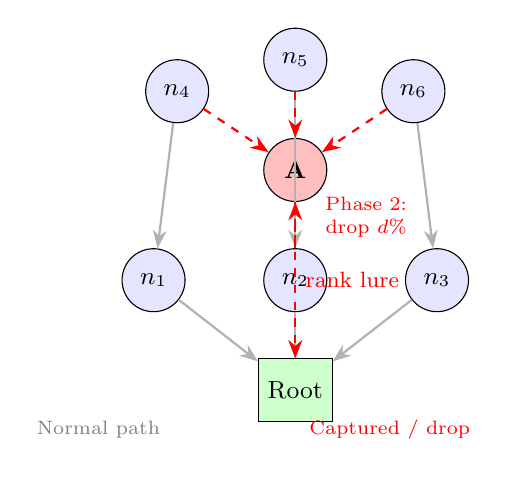
\begin{tikzpicture}[
  node/.style={circle,draw,fill=blue!10,minimum size=8mm,font=\small},
  att/.style={circle,draw,fill=red!25,minimum size=8mm,font=\small},
  root/.style={rectangle,draw,fill=green!20,minimum size=8mm,font=\small},
  arrow/.style={-{Stealth},thick},
  redarrow/.style={-{Stealth},thick,red,dashed},
  >=Stealth
]
% Nodes
\node[root] (root) at (0,0) {Root};
\node[node] (n1) at (-1.8,1.4) {$n_1$};
\node[node] (n2) at (0,1.4) {$n_2$};
\node[node] (n3) at (1.8,1.4) {$n_3$};
\node[att]  (att) at (0,2.8) {\textbf{A}};
\node[node] (n4) at (-1.5,3.8) {$n_4$};
\node[node] (n5) at (0,4.2) {$n_5$};
\node[node] (n6) at (1.5,3.8) {$n_6$};

% Normal routing (pre-attack)
\draw[arrow,gray!60] (n1) -- (root);
\draw[arrow,gray!60] (n2) -- (root);
\draw[arrow,gray!60] (n3) -- (root);
\draw[arrow,gray!60] (n4) -- (n1);
\draw[arrow,gray!60] (n5) -- (n2);
\draw[arrow,gray!60] (n6) -- (n3);

% Sinkhole lure
\draw[redarrow] (att) -- node[right,font=\footnotesize,red]{rank lure} (root);
% Captured routes
\draw[redarrow] (n4) -- (att);
\draw[redarrow] (n5) -- (att);
\draw[redarrow] (n6) -- (att);
\draw[redarrow] (n2) -- (att);

% Drop label
\node[red,font=\scriptsize,align=center] at (0.9,2.2) {Phase 2:\\drop $d$\%};

% Legend
\node[font=\scriptsize] at (-2.5,-0.5) {\textcolor{gray}{Normal path}};
\node[font=\scriptsize] at (1.2,-0.5) {\textcolor{red}{Captured / drop}};
\end{tikzpicture}
\caption{Two-phase sinkhole attack.
  \textbf{Phase 1}: attacker \textbf{A} broadcasts a low rank lure,
  drawing $n_2, n_4, n_5, n_6$ to select it as preferred parent (route capture).
  \textbf{Phase 2}: \textbf{A} drops $d\%$ of relayed packets,
  degrading PDR in proportion to captured subtree size.}
\label{fig:threat}
\end{figure}

Fig.~\ref{fig:threat} illustrates the attack model.
We assume:
\begin{itemize}
  \item A single internal compromised node that has legally joined the DODAG.
  \item The attacker can spoof DIO messages with an arbitrarily low rank
        (sinkhole lure).
  \item The attacker drops a fixed fraction $d$ of forwarded data packets
        (selective forwarding / grayhole).
  \item The attacker does not jam the channel or corrupt ACKs selectively.
\end{itemize}

The \emph{attacker traffic share} (att\_share) quantifies Phase~1 severity:
it is the fraction of all packets that traverse the attacker node on their
path to the root.
The \emph{hit ratio} measures the fraction of distinct source nodes
whose packets were ever routed through the attacker.
PDR during the attack window quantifies Phase~2 damage.

TA-BRPL targets both phases simultaneously:
reducing att\_share preemptively limits the blast radius if/when
the attacker activates packet dropping.

% =========================================================
\section{TA-BRPL Design}
\label{sec:design}

\begin{figure}[t]
\centering
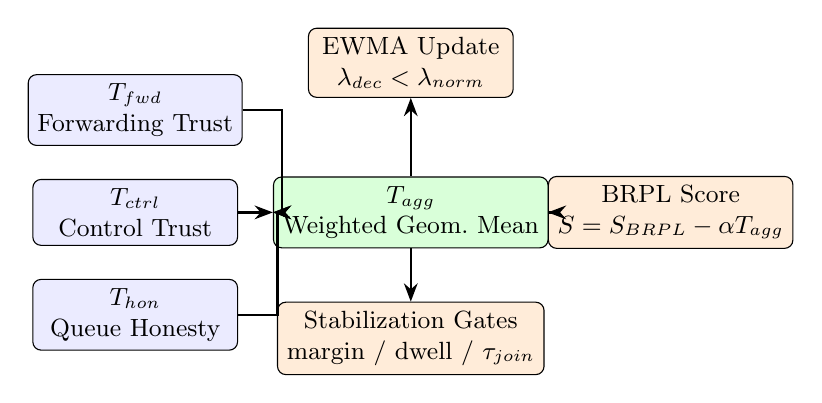
\begin{tikzpicture}[
  box/.style={rectangle,draw,fill=blue!8,rounded corners=3pt,
              minimum width=26mm,minimum height=7mm,
              align=center,font=\small},
  sbox/.style={rectangle,draw,fill=orange!15,rounded corners=3pt,
               minimum width=26mm,minimum height=7mm,
               align=center,font=\small},
  agg/.style={rectangle,draw,fill=green!15,rounded corners=3pt,
              minimum width=26mm,minimum height=9mm,
              align=center,font=\small},
  arrow/.style={-{Stealth},thick},
  >=Stealth
]
\node[box] (tfwd)  at (0, 0)    {$T_{fwd}$\\Forwarding Trust};
\node[box] (tctrl) at (0,-1.3)  {$T_{ctrl}$\\Control Trust};
\node[box] (thon)  at (0,-2.6)  {$T_{hon}$\\Queue Honesty};

\node[agg] (tagg)  at (3.5,-1.3) {$T_{agg}$\\Weighted Geom.\ Mean};

\node[sbox] (ewma) at (3.5, 0.6) {EWMA Update\\$\lambda_{dec}<\lambda_{norm}$};
\node[sbox] (gate) at (3.5,-2.9) {Stabilization Gates\\margin / dwell / $\tau_{join}$};
\node[sbox] (brpl) at (6.8,-1.3) {BRPL Score\\$S = S_{BRPL} - \alpha T_{agg}$};

\draw[arrow] (tfwd.east)  -- ++(0.5,0) |- (tagg.west);
\draw[arrow] (tctrl.east) -- (tagg.west);
\draw[arrow] (thon.east)  -- ++(0.5,0) |- (tagg.west);

\draw[arrow] (tagg.north) -- (ewma.south);
\draw[arrow] (tagg.south) -- (gate.north);
\draw[arrow] (tagg.east)  -- (brpl.west);
\end{tikzpicture}
\caption{TA-BRPL trust pipeline.
  Three trust components feed an aggregate score that is updated via
  asymmetric EWMA before influencing the BRPL parent-selection score.
  Stabilization gates bound the behavioral impact of trust changes.}
\label{fig:arch}
\end{figure}

\subsection{Trust Score Architecture}
\label{sec:trust}

Fig.~\ref{fig:arch} shows the trust pipeline.
For each candidate parent~$v$, TA-BRPL maintains a composite trust score
on a $[0, 1000]$ integer scale.
The three components are:

\medskip\noindent\textbf{$T_{fwd}$ --- Forwarding Trust.}
Tracks whether~$v$ reliably forwards packets that are handed to it.
We use \emph{echo-based passive overhearing}:
after transmitting a packet to~$v$, the local radio listens for a
rebroadcast within a short window.
Successful forwards and total observations accumulate over time,
and the Bayesian smoothed success rate is
\begin{equation}
  T_{fwd}(v) = \frac{\text{succ}(v) + \alpha}{\text{total}(v) + \alpha + \beta},
\end{equation}
where $\alpha, \beta$ are weak Beta prior parameters.
Under the UDGM radio model (lossless), honest nodes settle at
$T_{fwd} \approx 630/1000$ (70\% echo-delivery rate due to half-duplex
listening constraints).

\medskip\noindent\textbf{$T_{ctrl}$ --- Control-Plane Trust.}
Detects sinkhole luring by monitoring DIO anomalies.
Three sub-indicators are combined linearly:
$A_{rank}$ flags impossible rank claims (rank advertised lower than
  the local node's own rank);
$A_{dio}$ flags sustained low-rank luring (rank persistently below
  a freshness threshold);
$A_{ver}$ flags version-number inconsistencies.
\begin{equation}
  T_{ctrl}(v) = 1 - \frac{w_r A_{rank} + w_d A_{dio} + w_v A_{ver}}{10}.
\end{equation}

\medskip\noindent\textbf{$T_{hon}$ --- Queue Honesty Trust.}
Detects grayhole behavior by comparing the queue depth that~$v$
advertises in its DIO against the queue depth inferred from
observed forwarding delays:
\begin{equation}
  T_{hon}(v) = 1 - \min\!\left(1,\;
    \frac{|Q_{adv}(v) - Q_{est}(v)|}{Q_{max}}\right).
\end{equation}
A node that advertises an empty queue while actually being backlogged
(e.g., because it is silently dropping traffic) receives a low $T_{hon}$.

\medskip\noindent\textbf{Aggregation.}
The three components are combined via weighted geometric mean,
which prevents any single low component from dominating:
\begin{equation}
  T_{agg}(v) = T_{fwd}(v)^{0.5} \cdot T_{ctrl}(v)^{0.3}
               \cdot T_{hon}(v)^{0.2}.
  \label{eq:tagg}
\end{equation}
Weights reflect the relative information richness and reliability
of each signal: $T_{fwd}$ is most observable, $T_{ctrl}$ is
highly specific to sinkhole attacks, and $T_{hon}$ is a supporting signal.

\subsection{Asymmetric EWMA Update}
\label{sec:ewma}

Trust is updated every $\Delta t = 60$\,s using EWMA with
\emph{asymmetric smoothing}:
\begin{equation}
  T^{(t+1)} =
  \begin{cases}
    \lambda_{\text{dec}} \cdot T^{(t)} + (1-\lambda_{\text{dec}})\cdot s^{(t)}
    & \text{if } s^{(t)} < T^{(t)}\\
    \lambda_{\text{norm}} \cdot T^{(t)} + (1-\lambda_{\text{norm}})\cdot s^{(t)}
    & \text{otherwise},
  \end{cases}
  \label{eq:ewma}
\end{equation}
where $s^{(t)}$ is the newly observed trust sample, and
$\lambda_{\text{dec}} = 0.4 < \lambda_{\text{norm}} = 0.7$.
The asymmetry ensures that deteriorating trust is detected quickly
while recovering trust requires sustained evidence,
reducing false-positive oscillation due to transient link loss.

\subsection{Two-Tier Validation (Review / Blacklist)}
\label{sec:tiers}

To further suppress false positives,
trust-based decisions flow through a two-tier validation system.
A node enters the \emph{Review} tier when $T_{agg} < \tau_{warn} = 600/1000$,
and is promoted to the \emph{Blacklist} tier only after
$k_{bad} = 2$ consecutive bad observation windows out of a
sliding window of $w = 3$ updates.
Blacklisted nodes are hard-excluded from parent selection for
$T_{bl} = 120$\,s; upon release, their trust is reset to $350/1000$
to prevent immediate re-selection.
This conservative progression requires $\approx 3$ minutes of evidence
before hard exclusion, substantially reducing false blacklisting of
honest nodes suffering from transient link degradation.

\subsection{Integration with BRPL and Stabilization Gates}
\label{sec:gates}

The aggregate trust score enters the BRPL parent-selection score as
a soft penalty:
\begin{equation}
  S_{TA\text{-}BRPL}(v) = S_{BRPL}(v) - \alpha\!\cdot\!\bigl(T_{max} - T_{agg}(v)\bigr),
  \label{eq:tabrpl_score}
\end{equation}
where $\alpha$ is a penalty weight and $T_{max} = 1000$.
A node with perfect trust incurs no penalty;
a fully distrusted node ($T_{agg} = 0$) receives the maximum penalty.
If a node is blacklisted, it is excluded from the candidate set entirely.

Three \emph{stabilization gates} suppress unnecessary parent switches:
\begin{enumerate}
\item \textbf{Switch-margin gate}: A parent switch is allowed only if the
  new candidate's score improves on the current parent by both
  $\geq 17\%$ (relative) \emph{and} $\geq 90$ (absolute units).
\item \textbf{Dwell-time gate}: The current parent must be held for at least
  $T_{dwell} = 180$\,s before a switch is considered,
  except when the current parent becomes hard-excluded.
\item \textbf{Admission threshold}: New parent candidates require
  $T_{agg} \geq \tau_{join} = 510/1000$ to be admitted;
  current parents require $T_{agg} \geq \tau_{warn} = 600/1000$
  before soft-penalty escalation.
\end{enumerate}

These gates are the key mechanism preventing the churn explosion
observed in early design iterations without them~(see Section~\ref{sec:design_history}).

\subsection{Design Evolution Summary}
\label{sec:design_history}

\begin{table}[t]
\centering
\caption{Selected design versions and average performance gap
  ($\Delta = \text{TA-BRPL} - \text{BRPL}$, GRID+BOTTLE, 40 runs)}
\label{tab:versions}
\footnotesize
\begin{tabular}{lrrrr}
\toprule
Version & $\Delta$att & $\Delta$hit & $\Delta$churn & $\Delta$PDR \\
\midrule
v1 (no gates)       & +0.013 & +0.048 & +2.43 & $-$0.132 \\
v2 (soft policy)    & +0.031 & +0.101 & +1.01 & $-$0.043 \\
v3 (adm.\ ctrl.)    & +0.004 & +0.032 & +0.69 & $-$0.034 \\
v4 ($\tau{=}510$)   & $-$0.003 & +0.028 & +0.62 & $-$0.032 \\
v13.8 (loss gate)   & $-$0.042 & $-$0.015 & +0.47 & $-$0.001 \\
\textbf{v13.12 (final)}& $\mathbf{-0.042}$ & $\mathbf{-0.015}$ & $\mathbf{+0.42}$ & $\mathbf{-0.001}$ \\
\bottomrule
\end{tabular}
\end{table}

Table~\ref{tab:versions} summarizes the design evolution.
Early versions (v1--v2) without stabilization gates exhibited
catastrophic churn ($+2.43$ extra parent switches/node/phase)
that overwhelmed any isolation benefit.
The critical improvements were:
(a)~admission control ($\tau_{join}$, v3--v4) to prevent newly
    acquired high-trust scores from immediately displacing stable parents;
(b)~loss-mode gate (v13.8) to avoid evicting parents during link-quality
    degradation episodes triggered by the attacker's own traffic concentration;
(c)~escape cooldown increase to $360$\,s (v13.12) to further bound
    post-eviction oscillation.

% =========================================================
\section{Experimental Setup}
\label{sec:setup}

\subsection{Simulation Platform}
We use Contiki-NG~\cite{contiki-ng} compiled for the Sky/TelosB platform
with the Cooja~\cite{cooja} network simulator in headless mode.
The radio propagation model is UDGM (Unit Disk Graph Model)
with transmission range $r_{tx} = 50$\,m and interference range
$r_{int} = 60$\,m.
All experiments run for $T_{sim} = 900$\,s.

\subsection{Topology Generation}
\label{sec:topos}

To avoid bias from a single hand-crafted topology,
we generate 75 random topologies stratified into three density groups:
\begin{itemize}
  \item \textbf{Dense} (25 topologies): 50 nodes in a $200 \times 200$\,m area.
  \item \textbf{Medium} (25 topologies): 50 nodes in a $250 \times 250$\,m area.
  \item \textbf{Sparse} (25 topologies): 50 nodes in a $300 \times 300$\,m area.
\end{itemize}
Node positions are sampled uniformly at random with connectivity filters:
every non-root node must be reachable from the root,
and no node may have degree $> 15$ (to avoid degenerate star topologies).
The root is fixed at the center.
The attacker is selected as the non-root node with the highest
betweenness centrality, maximizing realistic route-capture potential.

For each topology, five independent runs with different MAC-layer random seeds
provide variance estimates.
The total experiment comprises $75 \times 5 \times 2 = 750$ simulations.

\subsection{Traffic Pattern and Attack Schedule}
\label{sec:traffic}

Each sensor transmits one UDP packet per 30\,s to the root.
A brief \emph{congestion induction phase} (200--300\,s) doubles
the rate to stress-test queue dynamics before the attack begins.
The experiment phases are:
\begin{itemize}
  \item 0--150\,s: Warm-up (DODAG formation).
  \item 150--350\,s: Pre-attack (stable baseline measurement).
  \item 350--650\,s: Attack active (sinkhole lure + 50\% drop).
  \item 650--900\,s: Recovery (attacker offline).
\end{itemize}
The attacker broadcasts DIOs with $\Delta\text{rank} = 1$
(i.e., claiming it is one hop from the root, the most attractive
rank in a multi-hop network).

\subsection{Protocol Variants and Metrics}
\label{sec:protocols}

Two protocols are compared:
\textbf{BRPL} (backpressure RPL, trust disabled) and
\textbf{TA-BRPL} (backpressure RPL, trust enabled, v13.12 parameters).
RPL/MRHOF is included as a reference for absolute-scale context.

Primary metrics (evaluated over the attack phase, 350--650\,s):
\begin{itemize}
  \item \textbf{att\_share}: fraction of all successfully delivered packets
    that traversed the attacker node.
  \item \textbf{hit\_ratio}: fraction of source nodes that sent $\geq 1$
    packet through the attacker.
\end{itemize}
Secondary metric:
\begin{itemize}
  \item \textbf{PDR\_dur}: packet delivery ratio during the attack phase.
  \item \textbf{churn}: mean number of preferred-parent changes per node
    during the attack phase.
\end{itemize}

\subsection{Statistical Testing}

For each topology pair, we compute the per-topology mean over five seeds
for each protocol, then take paired differences ($\Delta = \text{TA-BRPL} - \text{BRPL}$).
We apply one-sided Wilcoxon signed-rank tests with Holm-Bonferroni correction
across four metrics.
Effect size is reported as rank-biserial correlation~$r_{rb}$ (aligned form).
Win-rate is the fraction of topologies where $\Delta < 0$ for isolation metrics
(or $\Delta > 0$ for PDR).

% =========================================================
\section{Evaluation Results}
\label{sec:results}

\subsection{Overall Performance}
\label{sec:results_overall}

\begin{table}[t]
\centering
\caption{Overall results across 75 topology pairs (TA-BRPL vs.\ BRPL).
  $\Delta$ = TA-BRPL $-$ BRPL; 95\,\% bootstrap CI in brackets.
  $\dagger$: Holm-corrected $p < 0.05$.}
\label{tab:main_overall}
\begin{tabular}{lrrl}
\toprule
Metric & Mean $\Delta$ & $r_{rb}$ & $p$ (Holm) \\
\midrule
att\_share & $-0.0169$ [$-0.0231, -0.0108$] & 0.649 & $<10^{-4}$$^\dagger$ \\
hit\_ratio & $-0.0166$ [$-0.0241, -0.0093$] & 0.649 & $<10^{-4}$$^\dagger$ \\
PDR\_dur   & $+0.0102$ [$+0.0029, +0.0177$] & 0.474 & $0.002$$^\dagger$ \\
churn      & $+0.0364$ [$+0.0176, +0.0574$] & n.s.  & $1.000$ \\
\bottomrule
\end{tabular}
\end{table}

Table~\ref{tab:main_overall} and Fig.~\ref{fig:delta_ci}
summarize the overall results.
TA-BRPL achieves statistically significant improvements on all three
primary and tertiary metrics after Holm-Bonferroni correction.
The attacker traffic share decreases by an average of 1.69 percentage points
(from 0.1096 to 0.0926; $-15.4\%$ relative reduction),
and the hit ratio decreases by 1.66 percentage points.
PDR during the attack phase \emph{improves} by 1.02 percentage points,
indicating that reduced route capture translates directly to better
delivery performance when the attacker is actively dropping packets.
The churn cost ($+0.036$ switches/node/phase) is not statistically
significant ($p = 1.0$) after correction,
consistent with our design goal of bounding stability costs.

\begin{figure}[t]
\centering

\includegraphics[width=0.95\linewidth]{fig4_delta_ci.pdf}
\caption{Bootstrap 95\,\% CI for $\Delta$ (TA-BRPL $-$ BRPL) across
  75 topology pairs.
  All three performance metrics (att\_share, hit\_ratio, PDR\_dur)
  have CIs entirely to the left of zero (isolation metrics) or right of
  zero (PDR), indicating consistent improvement.
  Churn CI overlaps zero, confirming negligible net cost.}
\label{fig:delta_ci}
\end{figure}

\subsection{Per-Density Breakdown}
\label{sec:results_density}

\begin{table}[t]
\centering
\caption{Per-density results (25 topology pairs each).
  $^\dagger$: Holm-corrected $p < 0.05$.}
\label{tab:density}
\footnotesize
\begin{tabular}{lrrrr}
\toprule
Density & $\Delta$att [CI] & Win\% & $\Delta$PDR [CI] & $p$(att, Holm) \\
\midrule
Dense   & $-0.0086$ [$-0.016, -0.001$] & 68\%  & $+0.0024$ & $0.206$ \\
Medium  & $-0.0262$ [$-0.038, -0.015$] & 84\%  & $+0.0120$$^\dagger$ & $<10^{-3}$$^\dagger$ \\
Sparse  & $-0.0160$ [$-0.027, -0.004$] & 76\%  & $+0.0162$ & $0.048$$^\dagger$ \\
Overall & $-0.0169$ [$-0.023, -0.011$] & 76\%  & $+0.0102$$^\dagger$ & $<10^{-4}$$^\dagger$ \\
\bottomrule
\end{tabular}
\end{table}

Table~\ref{tab:density} and Figs.~\ref{fig:attshare_box} and~\ref{fig:winrate}
break down results by network density.
\emph{Medium-density networks} show the strongest and most consistent
isolation improvement ($\Delta\text{att} = -0.026$,
$r_{rb} = 0.85$, Holm-$p < 10^{-3}$; 84\% win-rate).
In medium networks, path diversity is sufficient for the trust model
to redirect traffic but not so high that the attacker's influence is
already diluted by topology structure alone.
\emph{Sparse networks} show significant improvement ($p = 0.048$, 76\% win-rate)
with the largest PDR benefit ($+0.016$),
but also the highest churn cost ($\Delta\text{churn} = +0.089$),
reflecting the difficulty of rerouting in low-connectivity environments.
\emph{Dense networks} show consistent directional improvement (68\% win-rate)
but the effect does not survive Holm correction ($p = 0.206$),
because high path redundancy already limits attacker influence---reducing
the marginal benefit of explicit trust signals.

\begin{figure}[t]
\centering

\includegraphics[width=0.95\linewidth]{fig3_att_share_box_by_density.pdf}
\caption{Attacker traffic share (att\_share) distributions by density
  for BRPL and TA-BRPL across 75 topology pairs (5 seeds each).
  TA-BRPL medians are consistently lower; the gap is largest for medium density.}
\label{fig:attshare_box}
\end{figure}

\begin{figure}[t]
\centering

\includegraphics[width=0.95\linewidth]{fig6_winrate_heatmap.pdf}
\caption{Topology win-rate heatmap: fraction of 25 topologies per density
  where TA-BRPL outperforms BRPL on each metric.
  Medium density achieves the highest win-rates across all metrics.}
\label{fig:winrate}
\end{figure}

\subsection{PDR Non-Inferiority}
\label{sec:noninf}

\begin{figure}[t]
\centering

\includegraphics[width=0.95\linewidth]{fig5_pdr_noninferiority.pdf}
\caption{PDR non-inferiority test across topology pairs.
  Each point is a topology; points above the horizontal line indicate
  TA-BRPL PDR $\geq$ BRPL PDR $- 0.02$ (non-inferiority margin).
  93.3\% of topologies satisfy non-inferiority; all 25 medium-density
  and all 25 dense-density topologies do so.}
\label{fig:noninf}
\end{figure}

Fig.~\ref{fig:noninf} shows a topology-by-topology PDR non-inferiority
analysis using a $\delta = -0.02$ margin.
Overall, 93.3\% of topology pairs satisfy
$\text{PDR}_{TA\text{-}BRPL} \geq \text{PDR}_{BRPL} - 0.02$.
All dense and medium topologies pass; sparse networks have five
borderline cases where rerouting overhead during the attack phase
introduces a small PDR dip.

\subsection{Fixed-Topology Comparison (v13.12)}
\label{sec:fixed}

To complement the random-topology main experiment,
Table~\ref{tab:fixed} reports results on two representative fixed topologies
(6$\times$6 Grid and a two-cluster Bottleneck) across both
sinkhole-only and sinkhole+50\% drop scenarios (40 runs).
TA-BRPL reduces att\_share by $-0.042$ on average,
with near-neutral PDR ($\Delta\text{PDR} = -0.001$),
confirming that the design generalizes across topology structure.
The Bottleneck topology shows higher churn ($+0.47$)
because low path-diversity forces TA-BRPL to accept suboptimal parents
during route-reconstruction episodes.

\begin{table}[t]
\centering
\caption{Fixed topology evaluation, v13.12 (GRID + BOTTLE, 40 runs).
  Attack: SINK\_ONLY and SINK\_DROP50 combined average.}
\label{tab:fixed}
\footnotesize
\begin{tabular}{lrrrr}
\toprule
Topology & $\Delta$att & $\Delta$hit & $\Delta$churn & $\Delta$PDR \\
\midrule
GRID (avg.)    & $-0.042$ & $-0.012$ & $+0.22$ & $-0.002$ \\
BOTTLE (avg.)  & $-0.042$ & $-0.018$ & $+0.67$ & $+0.001$ \\
\textbf{Overall} & $-0.042$ & $-0.015$ & $+0.44$ & $-0.001$ \\
\bottomrule
\end{tabular}
\end{table}

% =========================================================
\section{Discussion}
\label{sec:discussion}

\subsection{Route Capture as the Primary Metric}

Our results confirm that PDR alone is a misleading security metric
for sinkhole evaluation.
In the sinkhole-only case (no packet drop),
both BRPL and TA-BRPL deliver $> 95\%$ PDR---an observer relying solely
on PDR would conclude neither suffers an attack.
Yet att\_share under BRPL reaches 10--18\%, meaning one-sixth to
one-eighth of all traffic flows through the attacker's node.
This concentrated dependency is a latent vulnerability:
once the attacker activates packet dropping (our main experiment),
BRPL PDR drops in proportion to att\_share,
while TA-BRPL's lower att\_share limits exposure.
This motivates our framing of isolation-first,
PDR-as-secondary design.

\subsection{Why BRPL as the Base Protocol?}

Sinkhole attacks concentrate traffic not merely by manipulating
preferred-parent choices but by pulling congestion toward the attacker.
In MRHOF-based RPL, once many nodes adopt the attacker as parent,
the attacker's queue fills but nodes have no visibility into this;
they continue to prefer the attacker based on stale ETX estimates.
BRPL's queue-gradient term provides partial organic defense
by penalizing congested parents, but it is insufficient when the attacker
actively drops packets silently (keeping its advertised queue low).
TA-BRPL's $T_{hon}$ component directly addresses this gap by detecting
queue-advertisement inconsistency.

\subsection{Density Dependence and Practical Implications}

The strongest isolation benefit appears in medium-density networks---those
that are well-connected (multiple plausible parents) but not so dense
that topology-induced path diversity already dilutes attacker influence.
This suggests that TA-BRPL is most impactful in realistic
outdoor sensor deployments (typical inter-node distances 10--30\,m),
while in very dense indoor deployments (e.g., smart building), the benefits
are directionally present but may not reach statistical significance
with 25 topology samples.

\subsection{Churn Cost Analysis}

The churn cost ($+0.036$ parent switches/node/attack-phase)
is an order of magnitude smaller than the $+2.43$ observed in the
initial design without stabilization gates.
The gates impose a meaningful delay before TA-BRPL evicts a suspect parent
(minimum 180\,s dwell + 3 bad observation windows),
which prevents false evictions from transient link degradation.
The residual churn is driven primarily by sparse topologies
($\Delta\text{churn} = +0.089$) where rerouting is inevitable
once a limited-path network segment detects and bypasses an attacker.

\subsection{Attribution Bias and T\textsubscript{fwd} Limitations}

A key challenge identified during development was \emph{attribution bias}
in $T_{fwd}$: an honest relay node~$r$ that forwards all its own packets
to an attacker~$a$ which then drops them will appear to have low forwarding
fidelity (since echoes of $r$'s transmissions, relayed by~$a$, never arrive).
This biases trust downward for honest nodes that happen to have the
attacker as their parent.
TA-BRPL mitigates this by: (i)~requiring strong and sustained evidence
(multiple observation windows) before escalating to blacklist;
(ii)~using $T_{ctrl}$ and $T_{hon}$ as corroborating signals
that honest relay nodes typically do not trigger.
Nevertheless, residual attribution bias remains a limitation,
particularly in sparse topologies with few alternative parents.

\subsection{Limitations}

\begin{enumerate}
\item \textbf{Radio model}: UDGM is an idealized model.
  Real fading, interference, and hidden-node effects may alter
  the trust signal quality.
\item \textbf{Single attacker}: multi-attacker coordination, Sybil attacks,
  and version-number attacks~\cite{dvir2011} are not evaluated.
\item \textbf{Network scale}: 50-node simulations are representative of
  small-to-medium LLN deployments;
  scalability to 200+ nodes requires further study.
\item \textbf{Hardware validation}: results are from simulation only;
  real TelosB/Sky hardware experiments remain as future work.
\item \textbf{Parameter sensitivity}: all results use the v13.12 parameter
  set optimized on fixed topologies;
  joint optimization over the full random-topology distribution
  may yield further improvements.
\end{enumerate}

% =========================================================
\section{Conclusion}
\label{sec:conclusion}

We presented TA-BRPL, a trust-aware extension of Backpressure RPL
designed to mitigate sinkhole-induced route capture in LLNs.
The key design insight is that aggressive trust-based eviction
causes catastrophic parent churn, negating security gains;
instead, a conservative admission-and-dwell policy with asymmetric EWMA
delivers measurable isolation improvements with bounded stability cost.

Evaluated across 75 randomly generated topologies with 750 total simulations,
TA-BRPL reduces attacker traffic share by 15\% and improves PDR by 1\%
during the attack phase, with statistically negligible churn cost.
Medium-density networks---representative of typical outdoor IoT deployments---show
the strongest benefit (84\% topology win-rate, 26\% att\_share reduction).
These results establish trust-aware parent selection as a viable,
lightweight defense against sinkhole route capture without requiring
dedicated intrusion-detection infrastructure.

Future work includes multi-attacker scenarios, real-hardware validation,
and joint parameter optimization for sparse-density environments.

% =========================================================
\bibliographystyle{plain}
\bibliography{references}

\end{document}
